
%(BEGIN_QUESTION)
% Copyright 2012, Tony R. Kuphaldt, released under the Creative Commons Attribution License (v 1.0)
% This means you may do almost anything with this work of mine, so long as you give me proper credit

Dette hel-pneumatiske kjelereguleringssystemet regulerer vannnivået inne i damptrommelen:

$$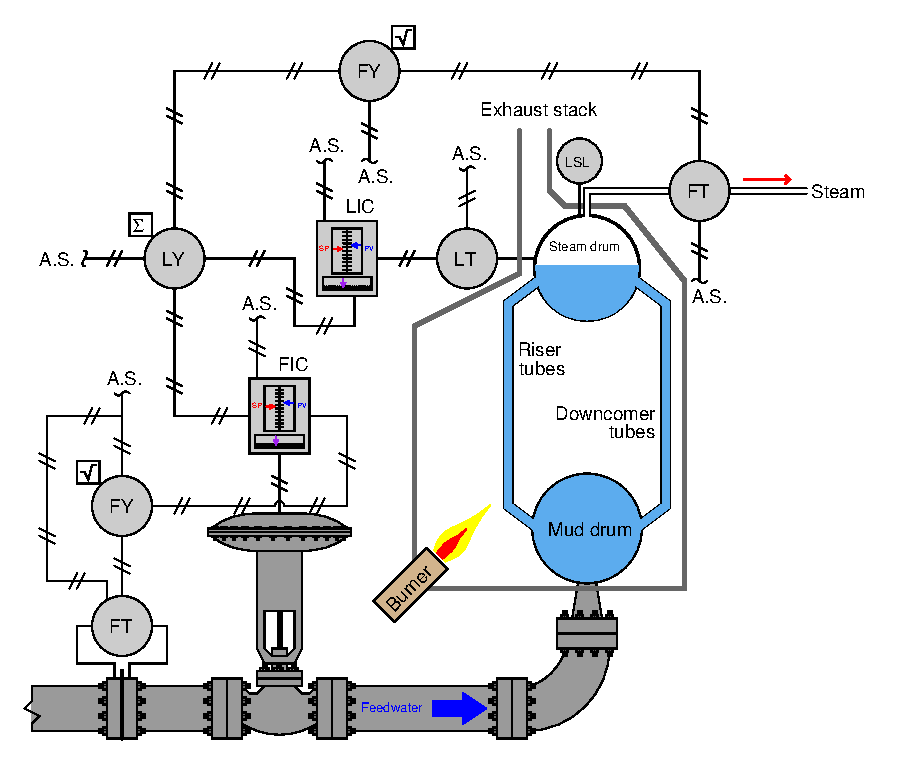
\includegraphics[width=15.5cm]{i01152x01.eps}$$

En dag ber ingeniøren i kjelhuset deg om hjelp til å senke vannnivået i damptrommelen mens kjelen er i drift. Vannnivået ligger normalt på 50\%, men han vil senke nivået til 35\% for å teste en lavnivå-vannalarmbryter som nylig er installert på trommelen. Det eneste problemet er at settpunktet på LIC ikke kan justeres, så det finnes ingen direkte måte å senke settpunktet for trommelnivået fra 50\% til 35\%. Verken LIC eller FIC har manuell modus.

\vskip 10pt

Finn en måte å ``lure'' reguleringssystemet til å senke vannnivået i trommelen i så lang tid som trengs for å gjennomføre testen, gitt at alle disse instrumentene er pneumatiske (mekaniske), noe som betyr at måleområdene kan justeres under drift med bare en skrutrekker. Vær konkret i beskrivelsen av løsningen, og forklar hvorfor den vil fungere.

\underbar{file i01152}
%(END_QUESTION)





%(BEGIN_ANSWER)

{\it Gi halv uttelling for løsninger som bare \underbar{midlertidig} senker vannnivået i damptrommelen.}

\vskip 10pt

Nivåtransmitteren (LT) må kalibreres om slik at den viser {\it 15\% høyere} nivå enn det som faktisk er i trommelen, slik at nivåregulatoren (LIC) arbeider for å senke vannnivået i trommelen (for å få LT-signalet tilbake til 50\% når reelt vannnivå er 35\%).

%(END_ANSWER)





%(BEGIN_NOTES)

{\bf Denne oppgaven er kun ment for prøver/eksamen, ikke arbeidsark!}.

%(END_NOTES)

